\chapter{Dataset}

\section{Geant4 Simulation}

Geant4 is a powerful and widely used simulation toolkit for modeling particle interactions with matter. It provides detailed simulations of detector geometry, material interactions, and physics processes, enabling accurate predictions of detector responses. In the CMS experiment, Geant4 plays a crucial role in validating experimental results and designing detector upgrades such as the High-Granularity Calorimeter (HGCal).

\subsection{Physics Processes}

Geant4 provides a comprehensive suite of physics processes covering electromagnetic,
hadronic, and optical interactions. For the HGCal, electromagnetic processes such as
ionization, bremsstrahlung, and photon interactions are particularly important in the
CE-E section, while hadronic processes are crucial for modeling particle showers in
the CE-H~\cite{geant4_toolkit}.

\subsection{Physics Processes}

Geant4 includes a comprehensive suite of physics processes covering electromagnetic, hadronic, and optical interactions. For the HGCal, electromagnetic processes such as ionization, bremsstrahlung, and photon interactions are particularly important in the CE-E section, while hadronic processes are crucial for modeling particle showers in the CE-H \cite{geant4_toolkit}.

\subsection{Geometry and Materials}

Geant4 enables users to define complex and highly detailed detector geometries with exceptional precision and flexibility. Taking the High-Granularity Calorimeter (HGCal) as an example, the arrangement of silicon sensors, scintillator tiles, and absorber plates is accurately modeled in Geant4. Each component is defined in terms of its precise geometry and physical properties, including parameters such as density, radiation length, and interaction cross-sections.

Through Geant4, the HGCal geometry is meticulously constructed layer by layer. Silicon sensors, segmented into hexagonal cells, simulate active regions where particles interact to generate measurable signals. Absorber materials like lead and steel are defined to induce particle showers, while scintillator tiles are incorporated to detect the resulting secondary particles. This level of detail ensures that simulations replicate real-world interactions, providing reliable data for performance optimization and physics studies.

\subsection{Applications in HGCal Development}

Geant4 has played a crucial role in optimizing the design of the HGCal. Through simulations of various configurations and material choices, researchers have fine-tuned the detector to achieve optimal performance in terms of energy resolution, granularity, and radiation tolerance. Additionally, these simulations aid in the development of reconstruction algorithms and calibration techniques specifically tailored to the unique characteristics of the HGCal~\cite{geant4_toolkit}.


Below is a demonstration of a Geant4 simulation for the HGCal, illustrating the interaction of a 20 GeV $\pi^{+}$ particle within the detector. An interesting aspect of Geant4 visualizations is the use of distinct colors to represent different particle types and interactions. In this simulation, charged particles are labeled in green, neutral particles in red, and interactions within the calorimeter in blue.


\begin{figure}[h]
    \centering
    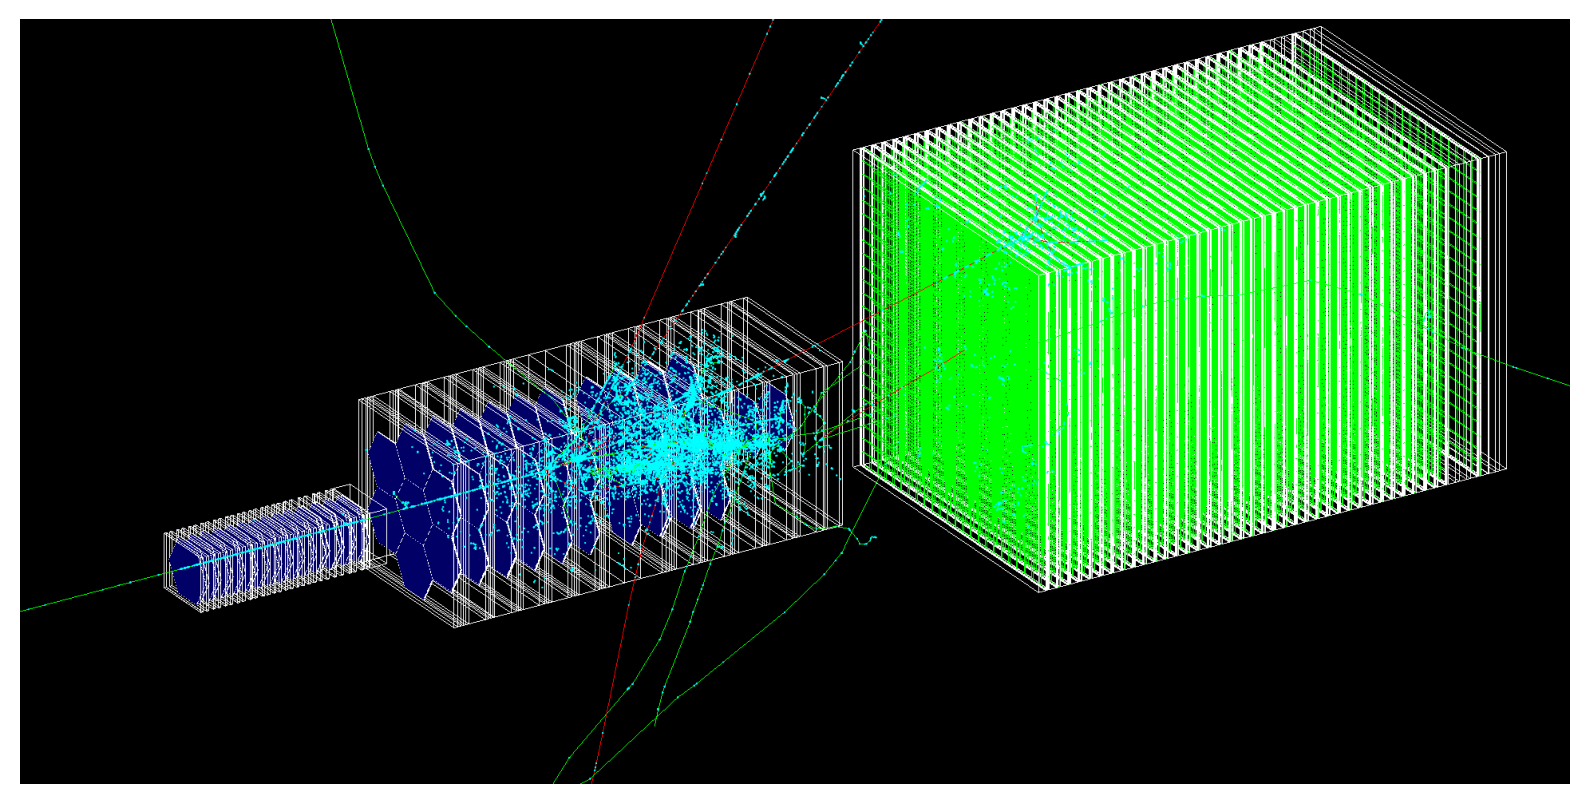
\includegraphics[width=\textwidth]{Figures/geant4_simulation.png}
    \caption{Visualization of a Geant4 simulation for the HGCal, showing particle showers in the calorimeter layers. (Image credit: Geant4 Collaboration)}~\cite{geant4_simulation}
    \label{fig:geant4_simulation}
\end{figure}

\subsection{Challenges of Geant4}

While Geant4 is a powerful and widely used simulation toolkit, it presents several challenges that impact its efficiency and usability in large-scale physics experiments.

\begin{itemize}
    \item \textbf{Computational Intensity:} \\
    Geant4 simulations require significant computational resources, particularly for high-energy physics experiments involving dense materials and complex interactions. The need to track billions of particles through detailed detector geometries makes large-scale simulations computationally expensive~\cite{geant4_reference}.
    
    \item \textbf{High Complexity:} \\
    The object-oriented design of Geant4 provides flexibility but also introduces a steep learning curve. Users must understand multiple modules, including geometry definitions, physics processes, and tracking systems, which can slow down the implementation of new simulations~\cite{geant4_doc}.
    
    \item \textbf{Scaling Issues:} \\
    With increasing experimental data rates, such as those expected in the High-Luminosity Large Hadron Collider (HL-LHC) phase, Geant4 faces challenges in maintaining simulation accuracy while keeping computational costs manageable. Machine learning approaches, such as diffusion models, are being explored as potential solutions to accelerate Geant4-like simulations while retaining high fidelity.
    
    \item \textbf{Validation and Maintenance:} \\
    Ensuring the accuracy of Geant4 requires continuous validation against experimental data. Physics models must be regularly updated and optimized to reflect the latest theoretical and experimental findings. Additionally, software maintenance and debugging add further complexity to large-scale implementations~\cite{geant4_validation}.
\end{itemize}

Despite these challenges, Geant4 remains an essential tool in particle physics and detector simulations, with ongoing research focusing on improving its computational efficiency and expanding its applicability to future high-energy physics experiments.


Geant4 remains an indispensable tool in the development and operation of the CMS detector, enabling detailed studies of particle interactions and supporting advancements in high-energy physics.

\section{The Fast Calorimeter Simulation Challenge (CaloChallenge)}

The Fast Calorimeter Simulation Challenge, or CaloChallenge, is an initiative designed to advance the development of fast, accurate, and efficient generative models for calorimeter shower simulations. This challenge bridges the gap between traditional simulation methods like GEANT4 and novel machine learning approaches, providing datasets, benchmarks, and metrics for evaluation~\cite{calochallenge}.

\subsection{Objectives}

CaloChallenge has the following primary goals:

\begin{itemize}
    \item Encourage the development of generative models capable of fast and accurate calorimeter shower simulation.
    \item Provide standardized datasets and metrics for consistent evaluation and benchmarking.
    \item Foster collaboration across the high-energy physics and machine learning communities.
\end{itemize}

\subsection{Datasets}

The CaloChallenge offers three distinct datasets, each increasing in complexity, to evaluate model performance in diverse scenarios. The datasets are as follows:

\subsubsection{Dataset 1: ATLAS GEANT4 Open Datasets}
Dataset 1 is based on simulations using the ATLAS detector geometry. It includes two single-particle shower types: photons and charged pions. The voxelized shower information is derived from single particles produced at the calorimeter surface in the $\eta$ range of 0.2-0.25. The detector geometry consists of 5 layers for photons and 7 layers for pions, with the number of radial and angular bins varying by layer and particle type.

\begin{itemize}
    \item Voxel structure:  
    \begin{itemize}
        \item 368 voxels for photons  
        \item 533 voxels for pions  
    \end{itemize}
    \item Incident energy levels: 15 discrete values, spanning 256 MeV to 4 TeV in powers of two.  
    \item Number of events: 10,000 per energy level, except at higher energies where limited statistics are available.
\end{itemize}

This dataset serves as a baseline for evaluating generative models on relatively simple detector geometries and energy distributions.

\subsubsection{Dataset 2: Multi-Layer Geometry with Electrons}
This dataset simulates electron showers in a concentric cylindrical calorimeter, which consists of:
\begin{itemize}
    \item 45 layers, each containing:
    \begin{itemize}
        \item Active material (silicon)
        \item Passive material (tungsten)
    \end{itemize}
    \item Voxel segmentation:
    \begin{itemize}
        \item 9 radial bins $\times$ 16 angular bins per layer
        \item Total: 6,480 voxels (45 $\times$ 16 $\times$ 9)
    \end{itemize}
    \item Incident energies: Sampled from a log-uniform distribution in the range 1 GeV to 1 TeV.
    \item Number of events: 100,000
\end{itemize}

This dataset introduces high-granularity segmentation, challenging models to accurately capture energy depositions across a complex detector geometry.

\subsubsection{Dataset 3: High-Granularity Calorimeter Geometry}
Dataset 3 extends the complexity of Dataset 2 by significantly increasing granularity:

\begin{itemize}
    \item 45-layer calorimeter with active (silicon) and passive (tungsten) material.
    \item Higher voxel segmentation:
    \begin{itemize}
        \item 18 radial bins $\times$ 50 angular bins per layer
        \item Total: 40,500 voxels (45 $\times$ 50 $\times$ 18)
    \end{itemize}
    \item Electron energies: Log-uniformly sampled between 1 GeV and 1 TeV.
    \item Number of events: 50,000
\end{itemize}

This dataset is specifically designed to evaluate the ability of generative models to generalize and simulate realistic high-granularity calorimeters, such as those planned for HL-LHC and future collider experiments.


\subsection{Data Format}

Each dataset is stored as one or more HDF5 files created using Python's \texttt{h5py} module with gzip compression. The files include:

\begin{itemize}
    \item \texttt{incident\_energies}: An array of shape (\texttt{num\_events}, 1) containing the incoming particle energies in MeV.
    \item \texttt{showers}: An array of shape (\texttt{num\_events}, \texttt{num\_voxels}) storing the energy depositions (in MeV) for each voxel, flattened in a specific order.
\end{itemize}

The mapping of voxel indices to spatial coordinates follows the detector segmentation. Helper functions are provided for reshaping and handling the data.

\subsection{Evaluation Metrics}

CaloChallenge evaluates the generative models using multiple metrics, including:

\begin{itemize}
    \item A binary classifier trained to distinguish between real GEANT4 samples and model-generated samples.
    \item Chi-squared comparisons between histograms of high-level features, such as layer energies and shower shapes.
    \item Speed and resource usage metrics, such as training time, generation time, and memory footprint.
    \item Interpolation capabilities to test generalization across unseen particle energies.
\end{itemize}

\subsection{Community Engagement}

Participants are encouraged to share their findings and contribute to community discussions. The challenge concludes with a workshop to present results, compare approaches, and collaborate on a community paper documenting the outcomes. For communication and updates, participants can join the ML4Jets Slack channel and the Google Groups mailing list.

For further details, visit the official CaloChallenge GitHub repository: \url{https://github.com/CaloChallenge/homepage}.

